% Autor: Leonhard Segger, Alexander Neuwirth
% Datum: 2017-10-30
\documentclass[
	% Papierformat
	a4paper,
	% Schriftgröße (beliebige Größen mit „fontsize=Xpt“)
	12pt,
	% Schreibt die Papiergröße korrekt ins Ausgabedokument
	pagesize,
	% Sprache für z.B. Babel
	ngerman
]{scrartcl}

% Achtung: Die Reihenfolge der Pakete kann (leider) wichtig sein!
% Insbesondere sollten (so wie hier) babel, fontenc und inputenc (in dieser
% Reihenfolge) als Erstes und hyperref und cleveref (Reihenfolge auch hier
% beachten) als Letztes geladen werden!

\usepackage{tikz}
\usetikzlibrary{calc,patterns,angles,quotes} % loads some tikz extensions\usepackage{tikz}
\usetikzlibrary{babel}

% Silbentrennung etc.; Sprache wird durch Option bei \documentclass festgelegt
\usepackage{babel}
% Verwendung der Zeichentabelle T1 (Sonderzeichen etc.)
\usepackage[T1]{fontenc}
% Legt die Zeichenkodierung der Eingabedatei fest, z.B. UTF-8
\usepackage[utf8]{inputenc}
% Schriftart
\usepackage{lmodern}
% Zusätzliche Sonderzeichen
\usepackage{textcomp}

% Mathepaket (intlimits: Grenzen über/unter Integralzeichen)
\usepackage[intlimits]{amsmath}
% Ermöglicht die Nutzung von \SI{Zahl}{Einheit} u.a.
\usepackage{siunitx}
% Zum flexiblen Einbinden von Grafiken (\includegraphics)
\usepackage{graphicx}
% Abbildungen im Fließtext
\usepackage{wrapfig}
% Abbildungen nebeneinander (subfigure, subtable)
\usepackage{subcaption}
% Funktionen für Anführungszeichen
\usepackage{csquotes}
\MakeOuterQuote{"}
% Zitieren, Bibliografie
\usepackage[sorting=none]{biblatex}


% Zur Darstellung von Webadressen
\usepackage{url}
%chemische Formeln
\usepackage[version=4]{mhchem}
% siunitx: Deutsche Ausgabe, Messfehler getrennt mit ± ausgeben
\usepackage{floatrow}
\floatsetup[table]{capposition=top}
\usepackage{float}
% Verlinkt Textstellen im PDF-Dokument
\usepackage[unicode]{hyperref}
% "Schlaue" Referenzen (nach hyperref laden!)
\usepackage{cleveref}
\sisetup{
	locale=DE,
	separate-uncertainty
}
\bibliography{BA-C-04_MP1_21-01-2019_References}

\begin{document}

	\begin{titlepage}
		\centering
		{\scshape\LARGE Versuchsbericht zu \par}
		\vspace{1cm}
		{\scshape\huge MP1 - Eigenschaften der Solarzelle \par} %TODO Iwie ist der Titel nur 50%
		\vspace{2.5cm}
		{\LARGE Gruppe BA-C-04 \par}
		\vspace{0.5cm}

		{\large Alexander Neuwirth (E-Mail: a\_neuw01@wwu.de) \par}
		{\large Leonhard Segger (E-Mail: l\_segg03@uni-muenster.de) \par}
		\vfill

		durchgeführt am 21.01.2019\par
		betreut von\par
		{\large Finn Kutschmann}

		\vfill

		{\large \today\par}
	\end{titlepage}
	\tableofcontents
	\newpage

	%TODO mehr TODO in Default

	\section{Kurzfassung}
	% Hypothese	und deren Ergebnis, wenn Hypothese ist, dass nur Theorie erfüllt, sagen: Erwartung: Theorie aus einführung (mit reflink) erfüllt
	% Ergebnisse, auch Zahlen, mindestens wenn's halbwegs Sinn ergibt
	% Was wurde gemacht
	% manche leute wollen Passiv oder "man", manche nicht

  \section{Theorie}
	% wdh. Texte
	% wdh. Besprechung
	\subsection{Dotierstoffe}
	\subsection{Solarzelle}
	\begin{equation}
			\label{eq_photostrom}
			I = I_0 \left[\exp{\left(\frac{eU}{n k_B T}\right)}-1\right]-I_{ph}
	\end{equation}

	\section{Methoden}
	% Bilder von der Website klauen
	% einer will Präsens

	\section{Ergebnisse und Diskussion}

	\subsection{Dotierstoffe}
	\subsubsection{Unsicherheiten}
	\subsubsection{Beobachtung und Datenanalyse}
	Mit der Vierspitzenmethode wurde der Widerstand $R=U/I$ gemessen.
	Daraus lässt sich dann mittels der Scheibendicke $d$ für dünne Scheiben ($d/s<0.5$, $s=\SI{1.59}{mm}$ Messspitzenabstand):
	\begin{equation}
			\rho = \frac{R d \pi}{\ln 2}
	\end{equation}
	\begin{equation}
			u(\rho) = \rho\cdot\sqrt{(u(R)/R)^2 + (u(d)/d)^2}
	\end{equation}
	Für die dickere Scheiben erhält man einen Korrekturfaktor gemäß DIN-NORM. %TODO cite DIN!
	Dieser beträgt für Probe 4 $0.84$ und für Probe 5 $0.83$.

	In \cref{tb_spez_wd} befinden sich die über mehrere Messungen gemittelten Messergebnisse.

	\begin{table}[H]
		\centering
		\begin{tabular}{c | c | c | c  }
			 &Widerstand $R$ in \si{\ohm}& Scheibendicke $d$ in \si{mm} & spez. Widerstand $\rho$ in \si{m\ohm m} \\ \hline
			 Probe 1, p-dot& \SI{50+-4}{}&\SI{0.4486+-0.0009}{}& \SI{101+-7}{} \\
			 Probe 2, n-dot&\SI{8.52+-0.21}{}&\SI{0.4532+-0.0009}{}&\SI{17.5+-0.4}{} \\
			 Probe 3, n-dot&\SI{0.0713+-0.0018}{}&\SI{0.0677+-0.001}{}&\SI{0.219+-0.005}{} \\
			 Probe 4, p-dot&\SI{0.00192+-0.00004}{}&\SI{1.999+-0.005}{}&\SI{0.0146+-0.0003}{} \\
			 Probe 6, n-dot&\SI{0.084+-0.007}{}&\SI{0.6826+-0.0009}{}&\SI{0.260+-0.022}{} \\
			 Probe 5, i-dot&\SI{25+-5}{}&\SI{2.1070+-0.0013}{}&\SI{199.2+-33.2}{}  \\ %TODO i-dot fine?
		\end{tabular}
		\caption{
		Silizium
		}
		\label{tb_spez_wd}
\end{table}
	\subsubsection{Diskussion}
	\subsection{Solarzelle}
	\subsubsection{Unsicherheiten}
	\subsubsection{Beobachtung und Datenanalyse}
	In \cref{fig_poly_unbeleuchtet_20} und \cref{fig_tandem_unbeleuchtet_20} sind die aufgenohmenen I-U-Kennlinien der polykistallinen Silizium Solarzelle und der Tandemzelle abgebildet.

	\begin{figure}[H]
			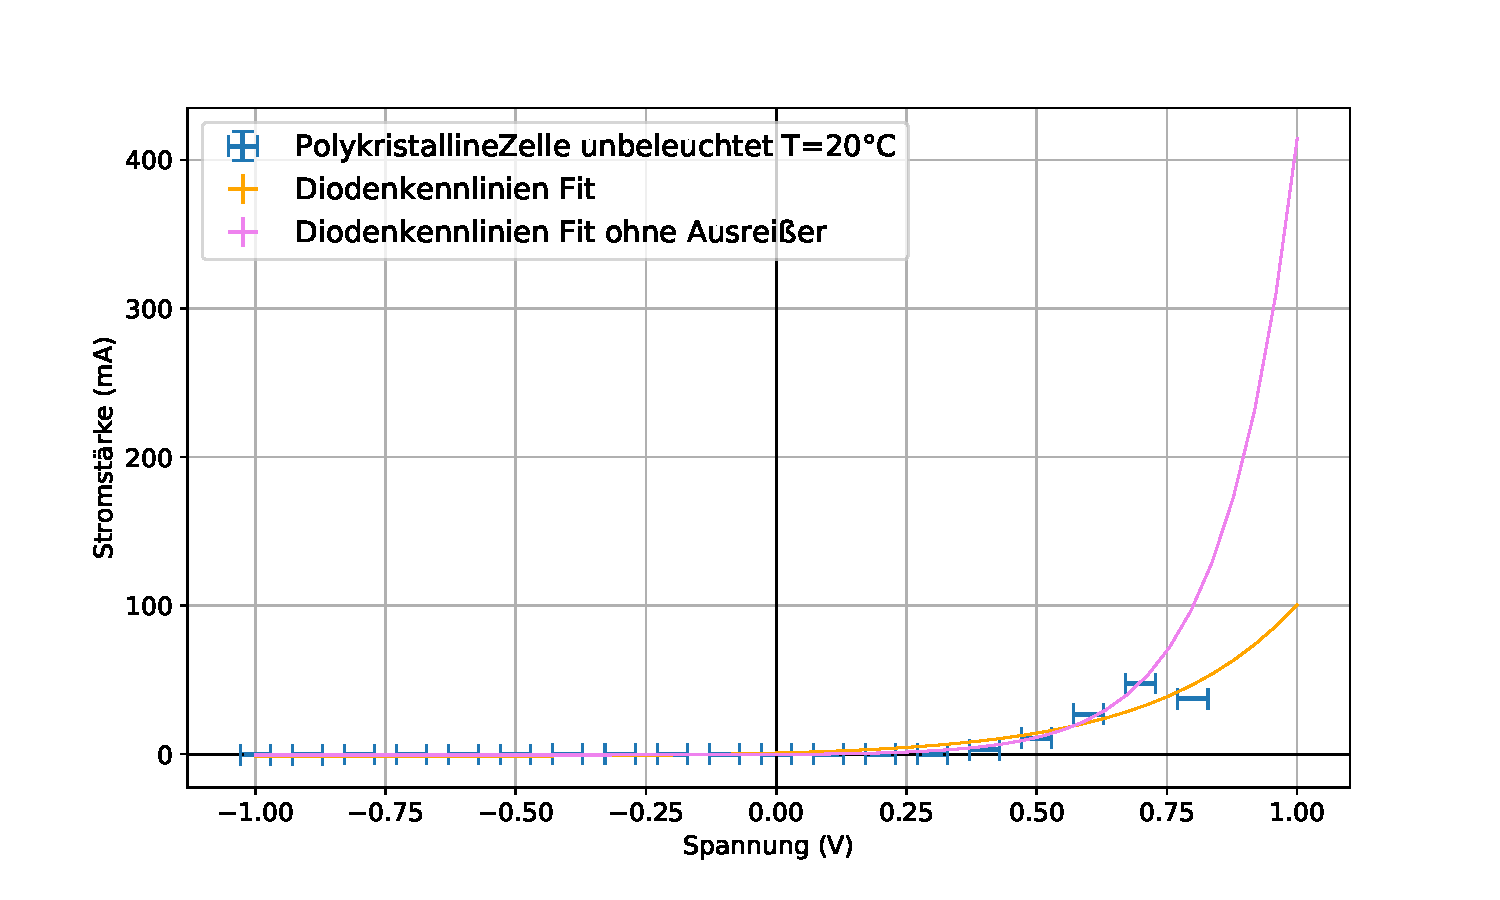
\includegraphics[width=.9\linewidth]{img/PolykristallineZelle_unbeleuchtet_20.pdf}
			\caption{
				I-U-Kennlinie einer polykristallinen Silizium Solarzelle bei Raumtemperatur.
								}
			\label{fig_poly_unbeleuchtet_20}
	\end{figure}

	\begin{figure}[H]
			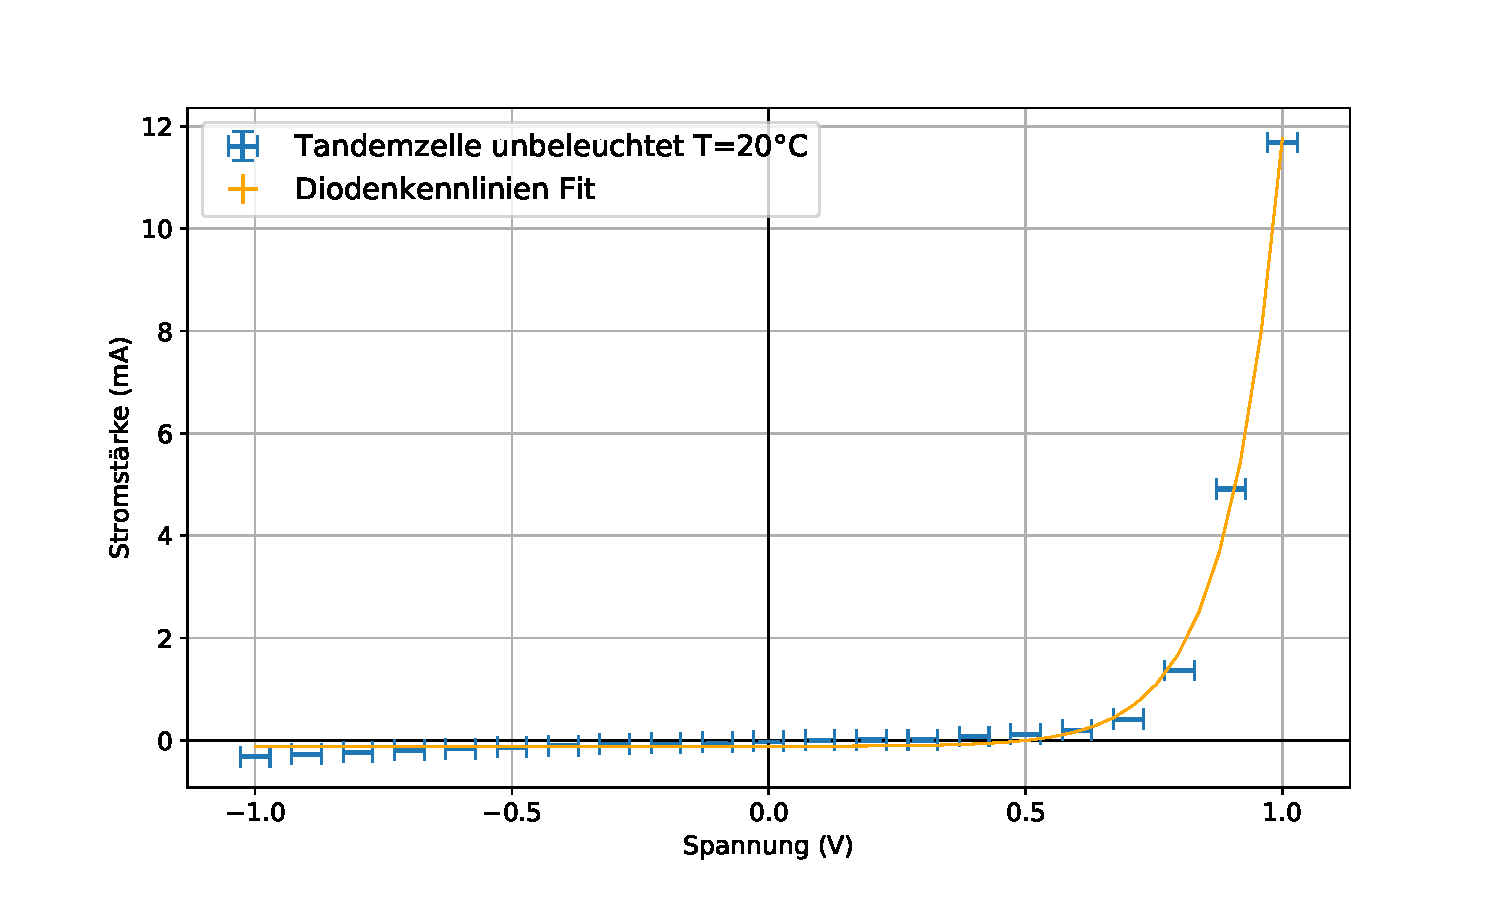
\includegraphics[width=.9\linewidth]{img/Tandemzelle_unbeleuchtet_20.pdf}
			\caption{
				I-U-Kennlinie einer Tandemzelle bei Raumtemperatur.
								}
			\label{fig_tandem_unbeleuchtet_20}
	\end{figure}

	Die Fitfunktion ist die ideale Diodenkennlinie unter Einstrahlung von Licht \cref{eq_photostrom}.

	\cref{fig_tandem_beleuchtet_20} stellt exemplarisch die I-U-Kennlinie der Solarzellen dar, wenn sie mit Licht bestrahlt werden (weitere befinden sich im \nameref{s_anhang}).
	Das rote (grüne) Rechteck gibt die im 4. Quadranten durch $U_{MPP}$ und $I_{MPP}$ ($U_{oc}$ und $I_{sc}$) begrenzte Fläche an.
	Die rote Fläche entspricht der Maximalen Leistung $P_{max} = U_{MPP}I_{MPP}$.
	Der Füllfaktor $FF$ ergibt sich als das Verhältnis der Flächen, also
	\begin{equation}
		FF = \frac{U_{mpp}I_{mpp}}{U_{oc}I_{sc}}.
	\end{equation}
	Dabei konnten $U_{MPP}$, $I_{MPP}$ und $I_{sc}$ direkt aus den Messpunkten extrahiert werden.
	$U_{oc}$ musste mittels des Fits interpoliert werden.


	\begin{figure}[H]
			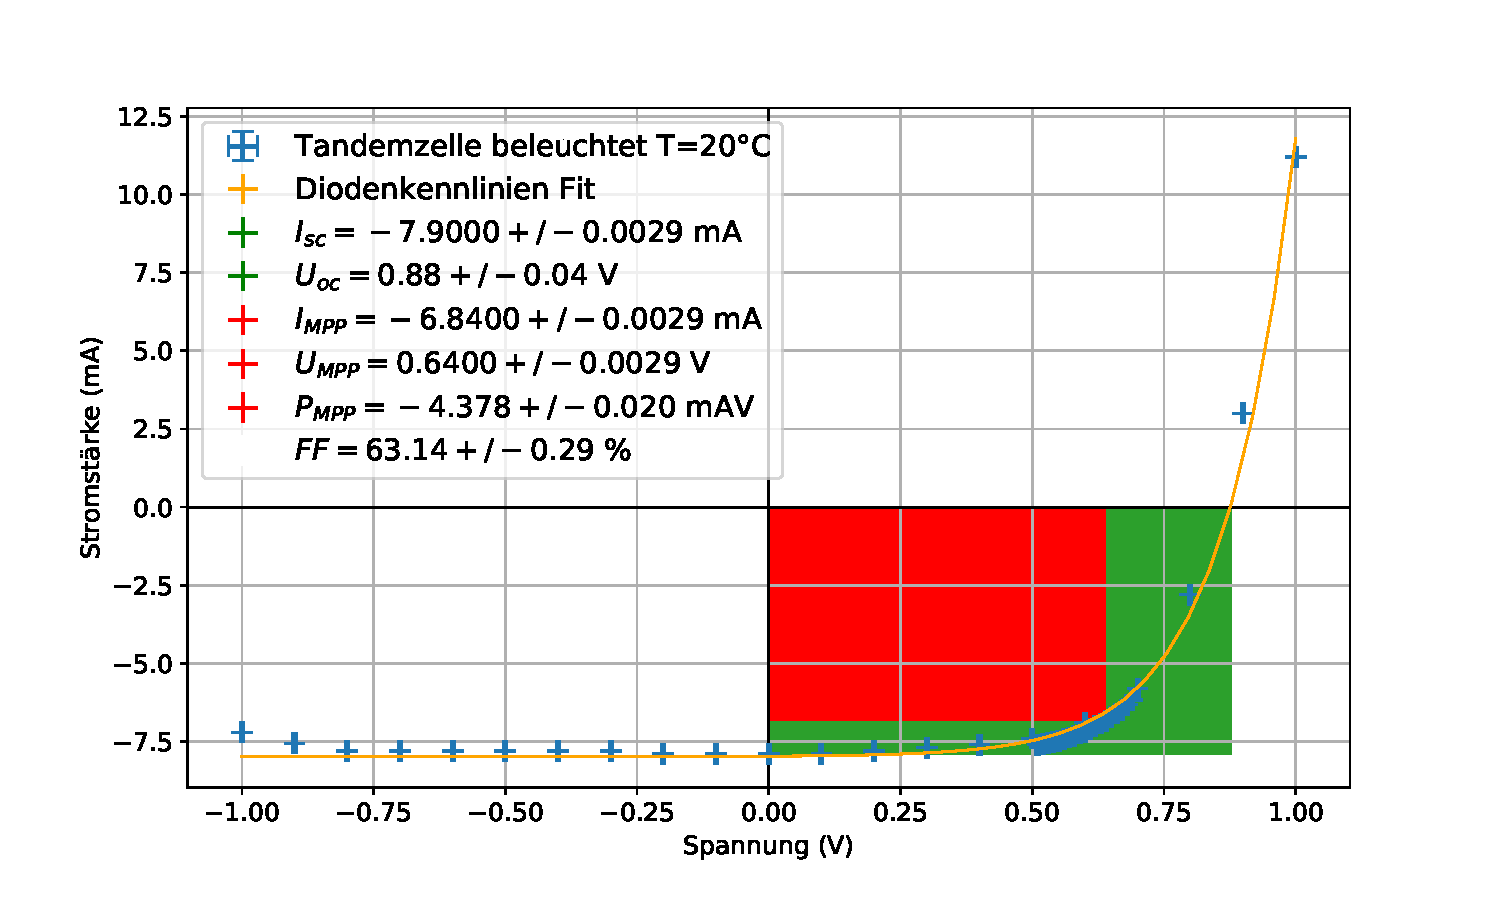
\includegraphics[width=.9\linewidth]{img/Tandemzelle_beleuchtet_20.pdf}
			\caption{
				I-U-Kennlinie einer Tandemzelle bei $T=\SI{20}{\celsius}$ unter Beleuchtung.
								}
			\label{fig_tandem_beleuchtet_20}
	\end{figure}
	%TODO table
	In \cref{tb_solar_param_poly} und \cref{tb_solar_param_tandem} sind die wichtigsten Parameter der Solarzellen die unter Variation der Temperatur bestimmt wurden aufgeführt.

\begin{table}[H]
	%TODO signums? alles positiv??
		\centering
		\begin{tabular}{c | c | c | c  }
			 &$T=\SI{20}{\celsius}$& $T=\SI{35}{\celsius}$& $T=\SI{50}{\celsius}$ \\ \hline
			 $I_{sc}$ in \si{mA}& \SI{151+-0.3}{}&\SI{149+-0.3}{}& \SI{147+-0.3}{} \\
			 $U_{oc}$ in \si{V}&\SI{0.63+-0.04}{}&\SI{0.61+-0.04}{}&\SI{0.61+-0.05}{} \\
			 $I_{MPP}$ in \si{mA}&\SI{108+-0.3}{}&\SI{99+-0.3}{}&\SI{96+-0.3}{} \\
			 $U_{MPP}$ in \si{V}&\SI{0.31+-0.003}{}&\SI{0.32+-0.003}{}&\SI{0.31+-0.003}{} \\
			 $P_{MPP}$ in \si{mW}&\SI{33.48+-0.32}{}&\SI{31.68+-0.3}{}&\SI{29.76+-0.3}{} \\
			 $FF$ in \si{\percent}&\SI{35.05+-2.5}{}&\SI{34.8+-2.5}{}&\SI{33+-2.7}{} \\
		\end{tabular}
		\caption{
		Polykristalline Zelle.
		}
		\label{tb_solar_param_poly}
\end{table}

\begin{table}[H]
	%TODO signums? alles positiv??
		\centering
		\begin{tabular}{c | c | c | c  }
			 &$T=\SI{20}{\celsius}$& $T=\SI{50}{\celsius}$& AM-Filter $T=\SI{20}{\celsius}$ \\ \hline
			 $I_{sc}$ in \si{mA}& \SI{7.9+-0.003}{}&\SI{5.42+-0.003}{}& \SI{0.94+-0.003}{} \\
			 $U_{oc}$ in \si{V}&\SI{0.88+-0.04}{}&\SI{0.776+-0.032}{}&\SI{0.705+-0.024}{} \\
			 $I_{MPP}$ in \si{mA}&\SI{6.84+-0.03}{}&\SI{4.24+-0.003}{}&\SI{0.700+-0.003}{} \\
			 $U_{MPP}$ in \si{V}&\SI{0.64+-0.003}{}&\SI{0.60+-0.003}{}&\SI{0.54+-0.003}{} \\
			 $P_{MPP}$ in \si{mW}&\SI{4.378+-0.022}{}&\SI{2.544+-0.012}{}&\SI{0.378+-0.003}{} \\
			 $FF$ in \si{\percent}&\SI{63.3+-2.8}{}&\SI{60.5+-2.5}{}&\SI{57+-2.0}{} \\
		\end{tabular}
		\caption{
		Tandemzelle.
		}
		\label{tb_solar_param_tandem}
\end{table}
	\subsubsection{Diskussion}
	%TODO Messfehler bei unbeleuchtet poly???? diskus
	%TODO hab das hier hin geschpoben weiel diskus
	Da in \cref{eq_photostrom} $I_{ph}$ der vertikale Verschiebung an der Ordinate entspricht, wird erwartet, dass dieser nahe Null ist, wenn die Solarzelle nicht beleuchtet wird, also in \cref{fig_poly_unbeleuchtet_20} und \cref{fig_tandem_unbeleuchtet_20}.
	%TODO passt bis auf thermo + hintergrund licht effekte


	% Allgemeine Beobachtungen
	% Einflüsse von veränderten Parametern auf Messung
	% Berechung nach Aufgabenstellung

	% Bezug/Nutzen oder sonst was
	% auch hier die Hypothese wiederholen
	% keine Messwerte hier, nach manchen Menschen, zumindest "direkt" erstellte Diagramme net hier, auch wenn Lesbarkeit-bla

	\section{Schlussfolgerung}
	% Rückgriff auf Hypothese und drittes Nennen dieser

	% Quellen zitieren, Websiten mit Zugriffsdatum
	% Verweise auf das Laborbuch (sind erlaubt)
	% Tabelle + Bilder mit Beschriftung
	%\printbibliography

	%TODO Anhang notwendig?
	\section{Anhang} \label{s_anhang}
	\subsection{Solarzelle}
	\begin{figure}[H]
			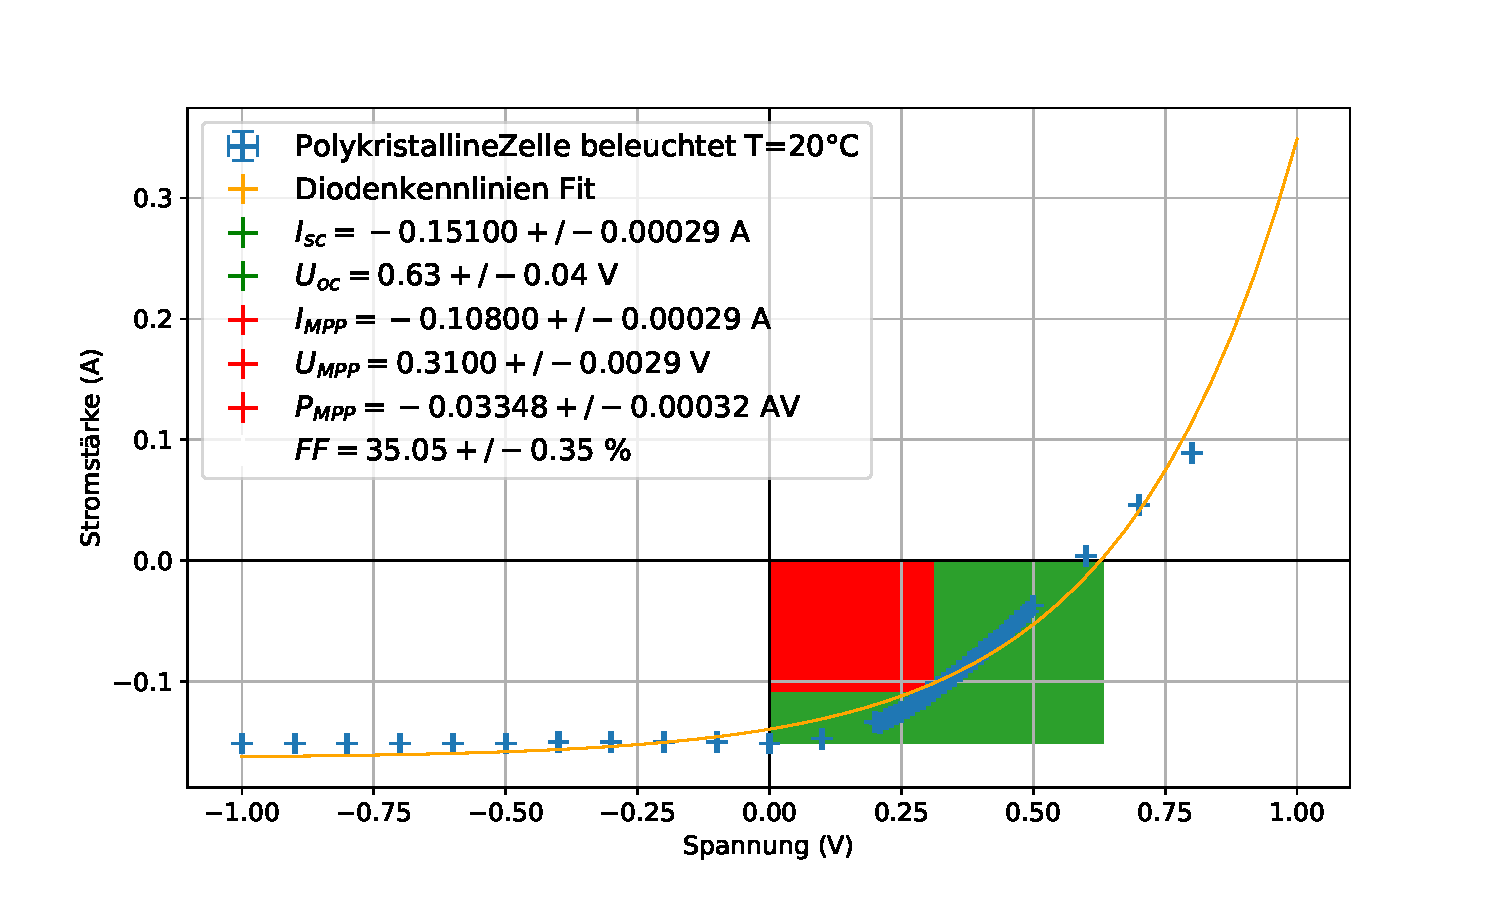
\includegraphics[width=.9\linewidth]{img/PolykristallineZelle_beleuchtet_20.pdf}
			\caption{
				I-U-Kennlinie einer polykristallinen Silizium Solarzelle bei Raumtemperatur unter Beleuchtung.
								}
			\label{fig_poly_beleuchtet_20}
	\end{figure}
	\begin{figure}[H]
			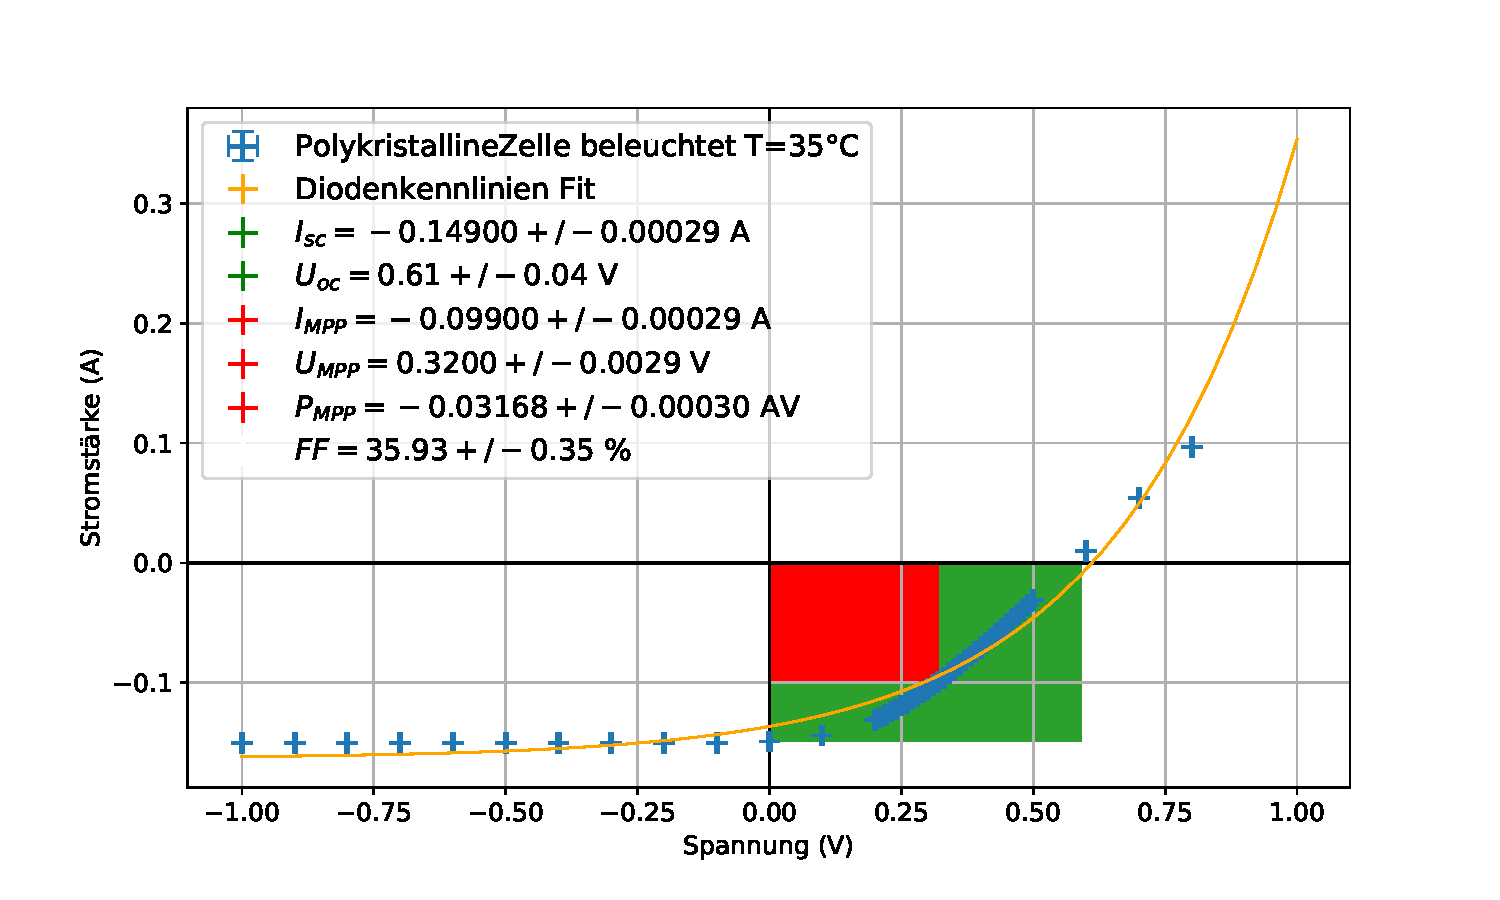
\includegraphics[width=.9\linewidth]{img/PolykristallineZelle_beleuchtet_35.pdf}
			\caption{
				I-U-Kennlinie einer polykristallinen Silizium Solarzelle bei $T=\SI{35}{\celsius}$ unter Beleuchtung.
								}
			\label{fig_poly_beleuchtet_35}
	\end{figure}

	\begin{figure}[H]
			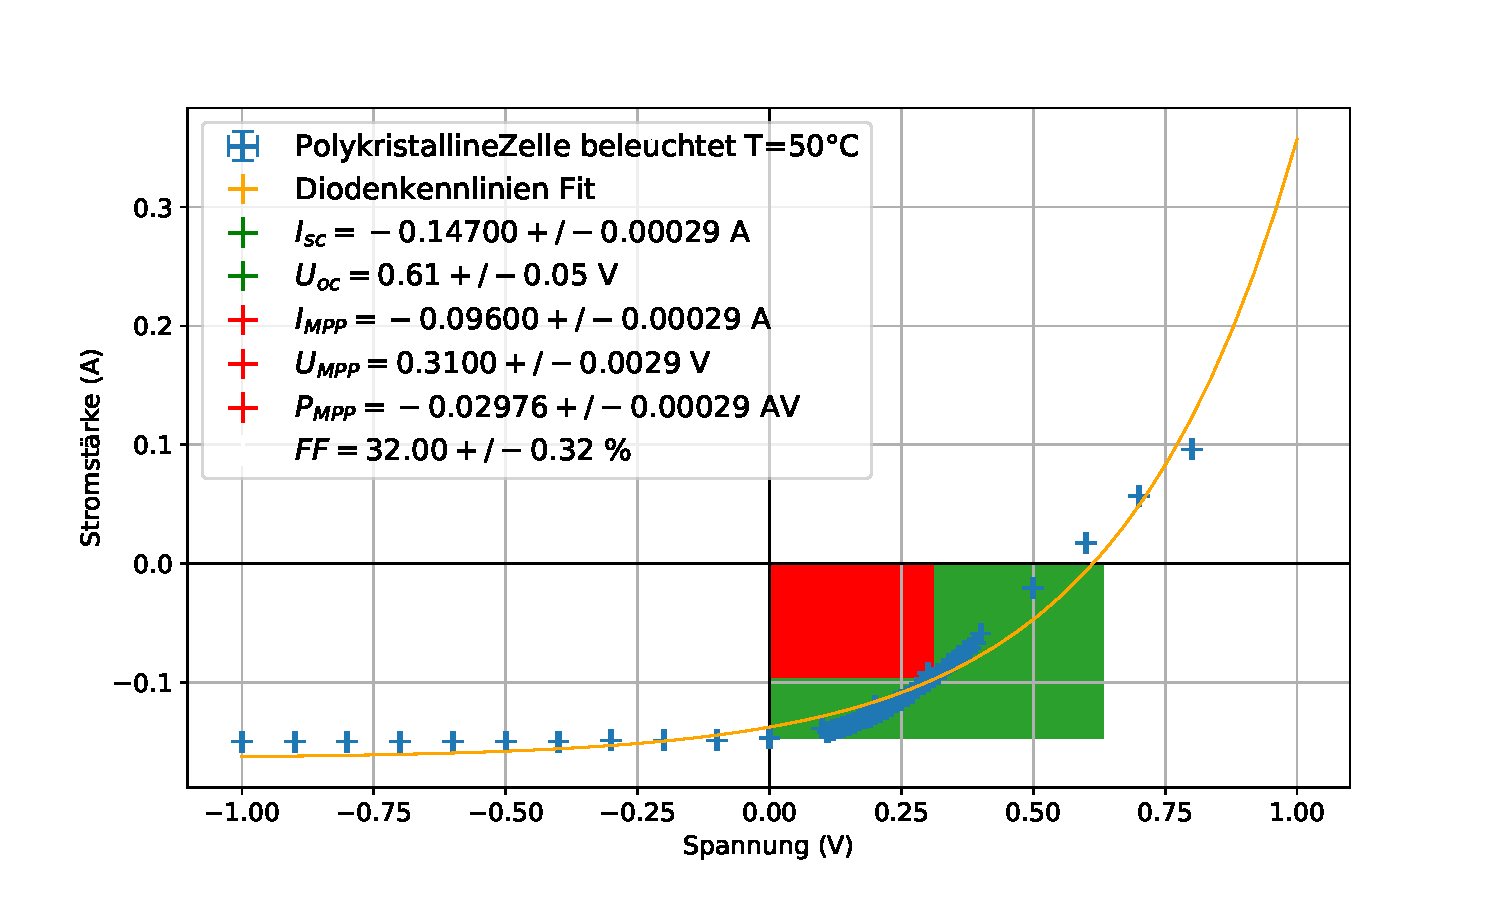
\includegraphics[width=.9\linewidth]{img/PolykristallineZelle_beleuchtet_50.pdf}
			\caption{
				I-U-Kennlinie einer polykristallinen Silizium Solarzelle bei $T=\SI{50}{\celsius}$ unter Beleuchtung.
								}
			\label{fig_poly_beleuchtet_50}
	\end{figure}


	\begin{figure}[H]
			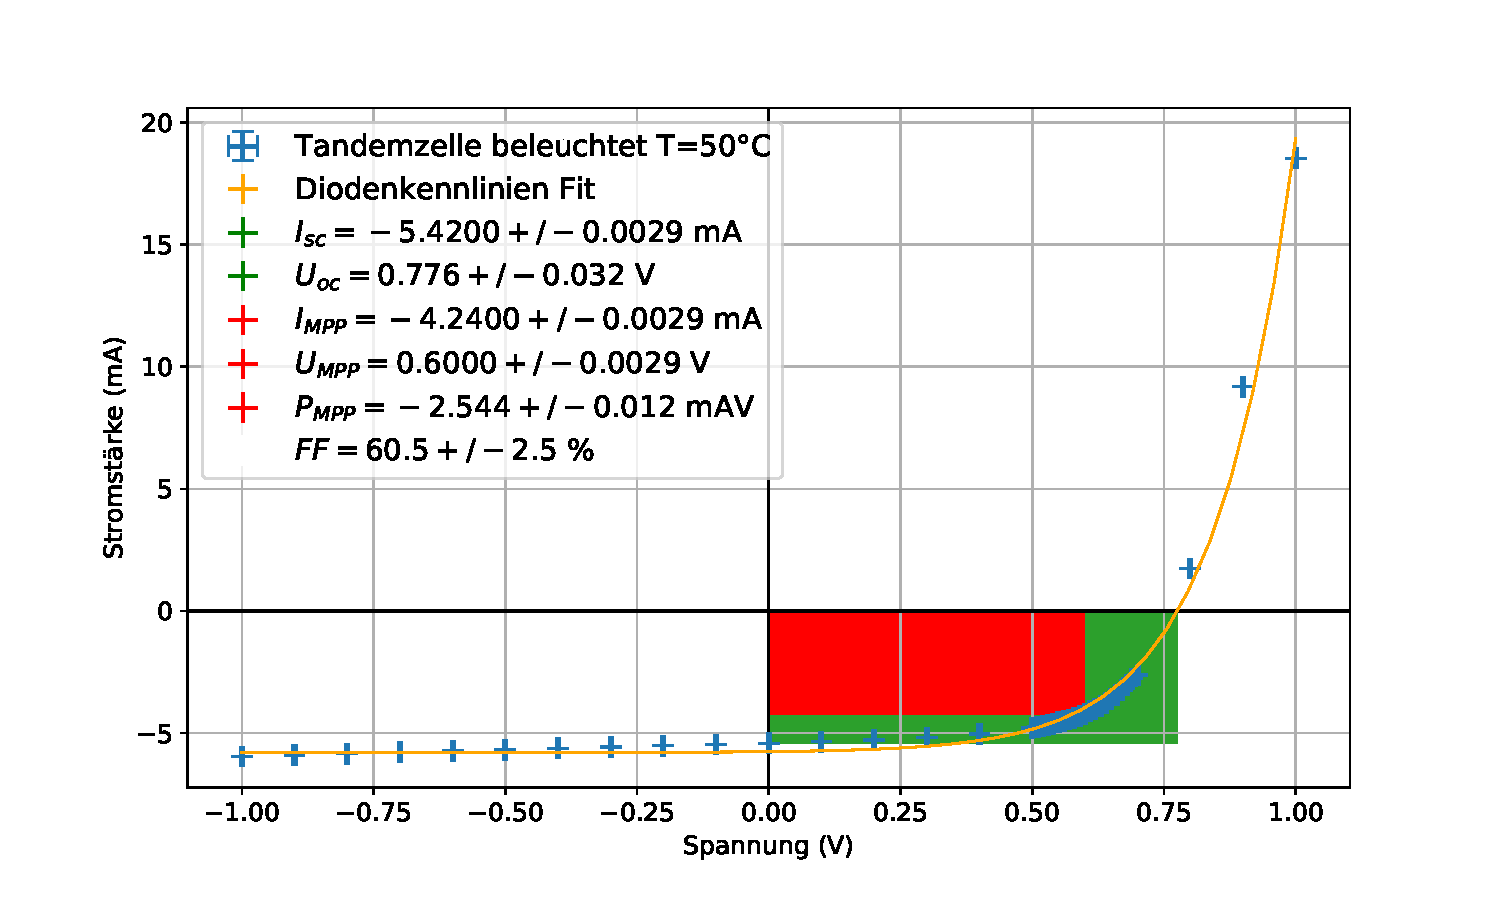
\includegraphics[width=.9\linewidth]{img/Tandemzelle_beleuchtet_50.pdf}
			\caption{
				I-U-Kennlinie einer Tandemzelle bei $T=\SI{50}{\celsius}$ unter Beleuchtung.
								}
			\label{fig_tandem_beleuchtet_50}
	\end{figure}

	\begin{figure}[H]
			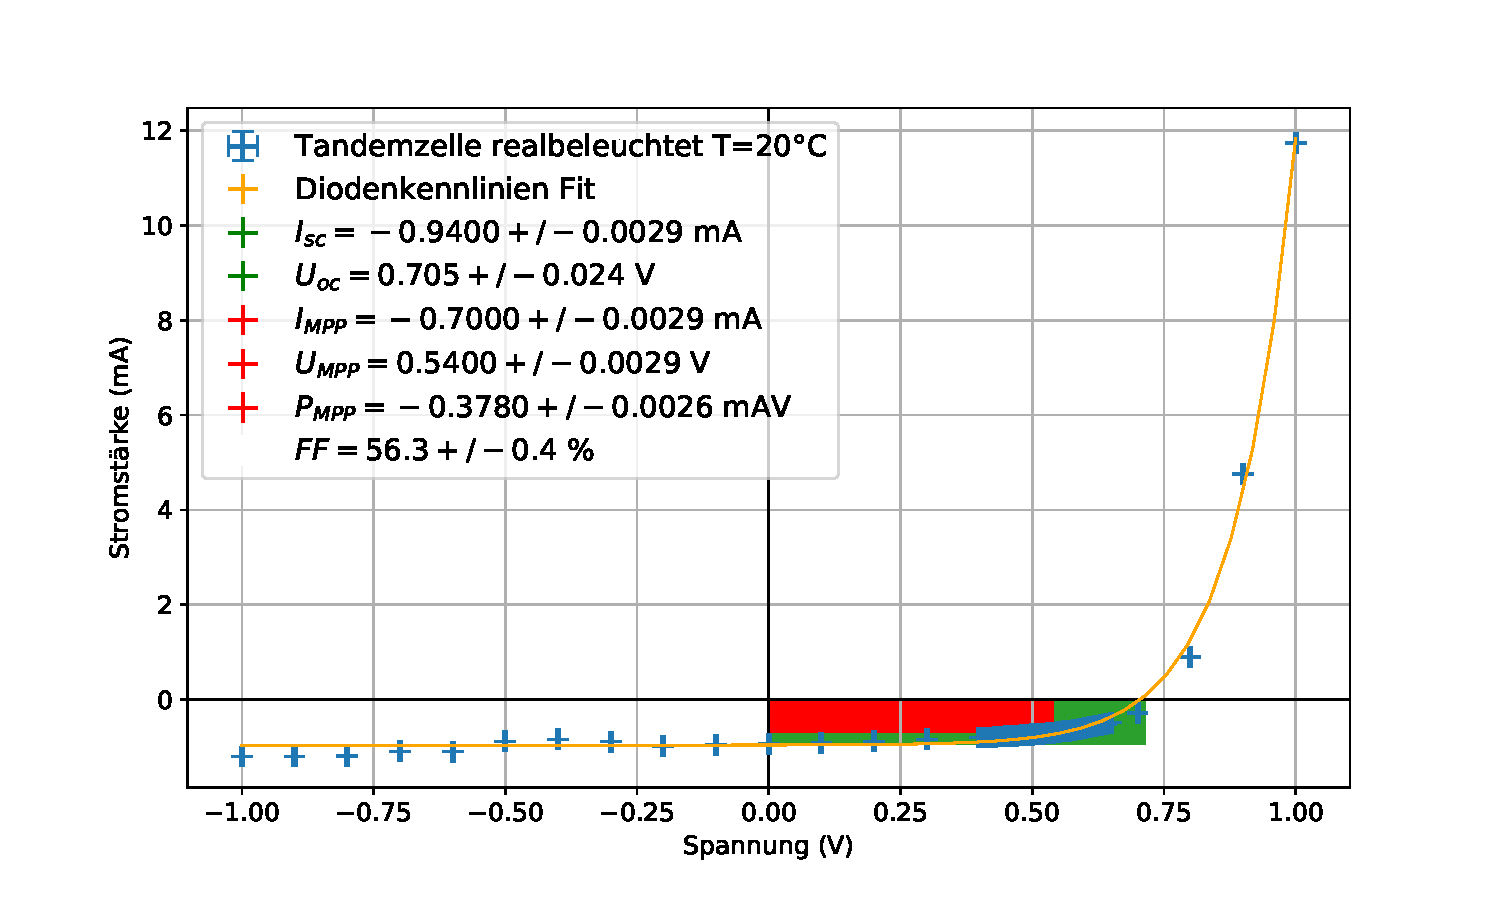
\includegraphics[width=.9\linewidth]{img/Tandemzelle_realbeleuchtet_20.pdf}
			\caption{
				I-U-Kennlinie einer Tandemzelle bei Raumtemperatur unter Beleuchtung durch einen AM-Filter.
				%TODO die Daten sagen nur hier "realbelecuhtet" also gehe ich von nur 1x AM-Filter aus
			}
			\label{fig_tandem_realbeleuchtet_20}
	\end{figure}
\end{document}
